% ---
\section{Random Forest}
% ---
Árvores são modelos presentes tanto em computação como estrutura de dados e em estatística como estrutura para tomadas de decisão. No contexto de aprendizado de máquina, a árvore de decisão refere-se a uma estrutura de modelo preditivo, um método de aprendizagem supervisionada não parametrizada utilizada para classificação e regressão (CART). Para \citeonline{HASTIE}, as árvores permitem um particionamento do espaço em um conjunto de retângulos com um modelo simple em cada. 

//por figura
Legenda
Neste exemplo \cite{HASTIE}, observa-se que o particionamento num espaço bidimensional, gerando 5 regiões. Ao lado, está a árvore que gerou esse particionamento.

Trata-se de uma representação de regras que dividem as observações em grupos com características em comum. Em geral, considera-se a hipótese de que cada característica possui um domínio finito e discreto.

\tikzset{
  treenode/.style = {shape=rectangle, rounded corners,
                     draw, align=center,
                     top color=white, bottom color=blue!20},
  root/.style     = {treenode, font=\Large, bottom color=purple!30},
  env/.style      = {treenode, font=\ttfamily\normalsize},
  dummy/.style    = {circle,draw}
}

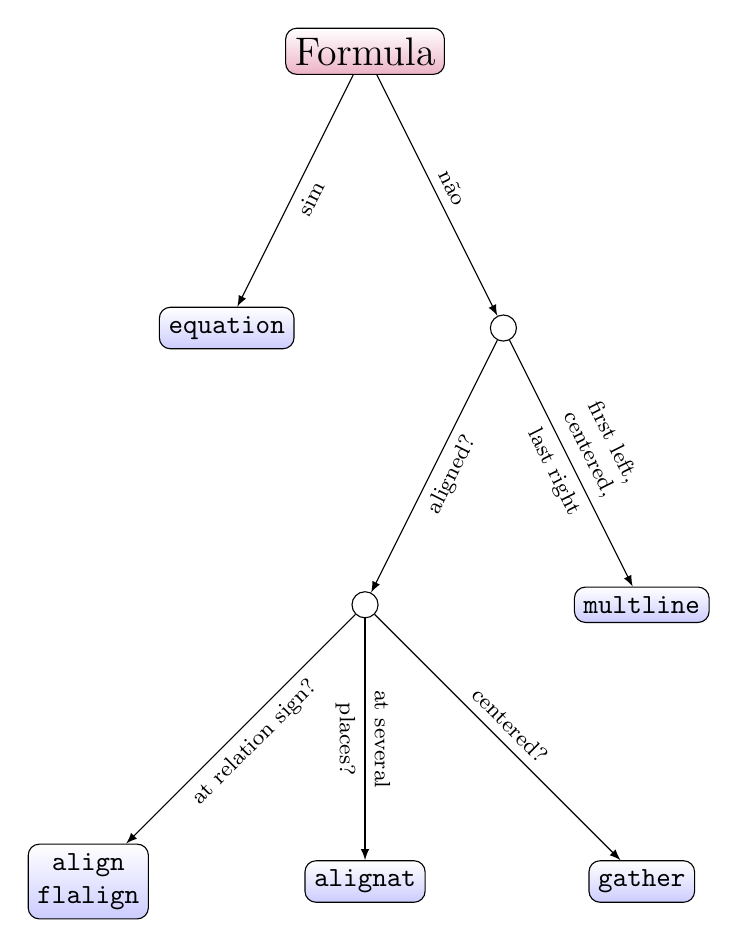
\begin{tikzpicture}
  [
    grow                    = down,
    sibling distance        = 10em,
    level distance          = 10em,
    edge from parent/.style = {draw, -latex},
    every node/.style       = {font=\footnotesize},
    sloped
  ]
  \node [root] {Formula}
    child { node [env] {equation}
      edge from parent node [below] {sim} }
    child { node [dummy] {}
      child { node [dummy] {}
        child { node [env] {align\\flalign}
          edge from parent node [below] {at relation sign?} }
        child { node [env] {alignat}
          edge from parent node [above] {at several}
                           node [below] {places?} }
        child { node [env] {gather}
                edge from parent node [above] {centered?} }
        edge from parent node [below] {aligned?} }
      child { node [env] {multline}
              edge from parent node [above, align=center]
                {first left,\\centered,}
              node [below] {last right}}
              edge from parent node [above] {não} };
\end{tikzpicture}

//legenda
Cada nó representa um atributo de um elemento da amostra. As folhas são consideradas a representação da classe a que uma observação pertence. Já o ramo é um conjunto de valores que reflete todas suas características e detalhes de um elemento.

Árvores de classificação


Seja \begin{math}p\end{math} os dados de entrada

Podemos representar de forma genérica o modelo da árvore de classificação por


Suponha que exista \begin{math}M\end{math} partição que possa ser divida em regiões \begin{math}R_{1}, R_{2}, ..., R_{M} \end{math} e que seja possível modelar a resposta para cada região com a constante \begin{math}c_{m}\end{math}, 

\begin{equation}
f(x) = \sum_{m=1}^{M}c_{m}I( x \in R_{m} )
\end{equation}

Utilizando como critério de minimização a soma do mínimos quadrados \begin{math}\sum{ (y_{i} - f(x_{i}))^{2}}\end{math}, temos que o melhor \begin{math}\hat c_{m}\end{math} é exatamente a média para \begin{math}y_{i}\end{math} na região \begin{math}R_{m}\end{math}:

\begin{equation}
\label{eq:media}
\hat c_{m} = m\acute edia(y_{i} | x_{i} \in R_{m})
\end{equation}

Para encontrar a melhor partição, é necessário recorrer a um algoritmo guloso.

Seja \begin{math}j\end{math} uma variável de reparticionamento, $s$ um ponto de divisão. É possível definir 1 par de semi planos 

\begin{equation}
R_{1}(j,s) = {X | X_{j}\leq s} \quad \textrm{e} \quad R_{2}(j,s) = {X | X_{j}\textgreater s})
\end{equation}

Resultando a busca pela de \begin{math}s\end{math} e \begin{math}j\end{math} que resolva

\begin{equation}
\min_{j,s} \left [ \min_{c_{1}} \sum_{x_{i} \in R_{1} (j,s)} (y_{i} - c_{1})^{2} + \min_{c_{1}} \sum_{x_{i} \in R_{2} (j,s)}(y_{i} - c_{2})^{2} \right ]
\end{equation} 


Mas como visto em \ref{eq:media}, temos que para qualquer $j$ e $s$, a minimização interna pode ser resolvida por:

\begin{equation}
\hat c_{1} = m\acute edia(y_{i} | x_{i} \in R_{1}(j,s)) \quad \textrm{e} \quad \hat c_{2} = m\acute edia(y_{i} | x_{i} \in R_{2}(j,s))
\end{equation} 

Este processo é repetido até que todas as regiões sejam descobertas.
